\documentclass[12pt,a4paper]{report}

% ── Packages ──────────────────────────────────────────────────────────────────
\usepackage[margin=1in]{geometry}
\usepackage{lmodern}
\usepackage{microtype}
\usepackage{hyperref}
\usepackage{booktabs}
\usepackage{longtable}
\usepackage{array}
\usepackage{tabularx}
\usepackage{listings}
\usepackage{xcolor}
\usepackage{graphicx}
\usepackage{titlesec}
\usepackage{fancyhdr}
\usepackage{amsmath}
\usepackage{amssymb}
\usepackage{enumitem}
\usepackage{tocloft}
\usepackage{setspace}
\usepackage{caption}
\usepackage[T1]{fontenc}
\usepackage[utf8]{inputenc}
\usepackage{float}
\usepackage{tikz}
\usetikzlibrary{shapes.geometric, arrows.meta, positioning, fit, backgrounds, calc, matrix}

% ── Colour palette ─────────────────────────────────────────────────────────────
\definecolor{darkblue}{RGB}{0,51,102}
\definecolor{midblue}{RGB}{0,102,153}
\definecolor{codeblue}{RGB}{0,70,150}
\definecolor{codegray}{RGB}{100,100,100}
\definecolor{codegreen}{RGB}{0,128,0}
\definecolor{codeback}{RGB}{245,245,245}
\definecolor{titleblue}{RGB}{0,51,102}

% ── TikZ figure styles ─────────────────────────────────────────────────────────
\tikzset{
    svcbox/.style={rectangle, rounded corners=4pt, draw=black!70, thick,
                   fill=gray!10, align=center, inner sep=6pt,
                   minimum height=1.1cm, font=\small},
    arrow/.style={-Stealth, thick, draw=black!70},
    edgelbl/.style={font=\scriptsize, fill=white, inner sep=2pt,
                    rounded corners=1pt, text=black},
    phase/.style={rectangle, draw=black!50, dashed, rounded corners=3pt,
                  fill=blue!4, inner sep=8pt, align=center},
    threatcap/.style={svcbox, text width=2.55cm, fill=red!6, draw=red!50},
    dmbox/.style={svcbox, text width=2.45cm, fill=green!6, draw=green!50!black},
    aitobs/.style={svcbox, text width=3.1cm, fill=midblue!12, draw=titleblue},
    gapother/.style={svcbox, text width=2.55cm, fill=gray!8},
    gapait/.style={svcbox, text width=2.85cm, fill=midblue!14, draw=titleblue, thick},
    fnbox/.style={svcbox, text width=3.35cm, font=\footnotesize, minimum height=1.25cm},
}

% ── Hyperref setup ─────────────────────────────────────────────────────────────
\hypersetup{
    colorlinks  = true,
    linkcolor   = titleblue,
    urlcolor    = codeblue,
    citecolor   = codeblue,
    pdftitle    = {AIT: Adversarial Integration Testing for SaaS APIs},
    pdfauthor   = {Adithya M N | Alaap V | Prajwal S | Nikhil Gowda T S}
}

% ── Code listing styles ────────────────────────────────────────────────────────
\lstdefinestyle{pythonstyle}{
    language         = Python,
    backgroundcolor  = \color{codeback},
    basicstyle       = \ttfamily\small,
    keywordstyle     = \color{codeblue}\bfseries,
    commentstyle     = \color{codegreen},
    stringstyle      = \color{codegray},
    numberstyle      = \tiny\color{codegray},
    numbers          = left,
    stepnumber       = 1,
    frame            = single,
    framerule        = 0.5pt,
    rulecolor        = \color{codegray},
    breaklines       = true,
    breakatwhitespace= false,
    tabsize          = 4,
    showstringspaces = false,
    captionpos       = b,
    aboveskip        = 10pt,
    belowskip        = 10pt,
    xleftmargin      = 2pt,
    xrightmargin     = 2pt
}

\lstdefinestyle{jsonstyle}{
    language         = {},
    backgroundcolor  = \color{codeback},
    basicstyle       = \ttfamily\small,
    frame            = single,
    framerule        = 0.5pt,
    rulecolor        = \color{codegray},
    breaklines       = true,
    captionpos       = b,
    aboveskip        = 10pt,
    belowskip        = 10pt,
    xleftmargin      = 2pt,
    xrightmargin     = 2pt
}

% ── Caption setup ──────────────────────────────────────────────────────────────
\captionsetup{
    font        = small,
    labelfont   = bf,
    labelsep    = period,
    skip        = 6pt
}
\captionsetup[figure]{position = bottom, name = Figure}
% Listings use their own caption= option (avoid captionsetup[lstlisting] --- breaks refs).

% ── Header / Footer ────────────────────────────────────────────────────────────
\setlength{\headheight}{14pt}
\pagestyle{fancy}
\fancyhf{}
\fancyhead[L]{\small AIT: Adversarial Integration Testing}
\fancyhead[R]{\small BIC685: Major Project Phase 1}
\fancyfoot[C]{\thepage}
\renewcommand{\headrulewidth}{0.4pt}

\fancypagestyle{plain}{
    \fancyhf{}
    \fancyhead[L]{\small\color{midblue}\textit{AIT: Adversarial Integration Testing for SaaS APIs}}
    \fancyhead[R]{\small\color{midblue}\textit{Major Project Phase 1 [BIC685]}}
    \fancyfoot[C]{\small\thepage}
    \renewcommand{\headrulewidth}{0.4pt}
    \renewcommand{\headrule}{%
        \hbox to\headwidth{\color{midblue}\leaders\hrule height\headrulewidth\hfill}
    }
}

% ── Section title formatting ───────────────────────────────────────────────────
\titleformat{\chapter}[block]
    {\normalfont\Large\bfseries\color{darkblue}}
    {\thechapter}{1em}{}
    [\vspace{2pt}\color{midblue}\titlerule]

\titleformat{\section}
    {\normalfont\large\bfseries\color{midblue}}
    {\thesection}{1em}{}

\titleformat{\subsection}
    {\normalfont\normalsize\bfseries\color{darkblue}}
    {\thesubsection}{1em}{}

\titlespacing*{\chapter}  {0pt}{-30pt}{16pt}
\titlespacing*{\section}  {0pt}{12pt}{6pt}
\titlespacing*{\subsection}{0pt}{8pt}{4pt}

% ── Misc ───────────────────────────────────────────────────────────────────────
\setlength{\parskip}{6pt}
\setlength{\parindent}{0pt}
\onehalfspacing

% ══════════════════════════════════════════════════════════════════════════════
\begin{document}

% ── Title Page ─────────────────────────────────────────────────────────────────
\begin{titlepage}
    \centering
    \vspace*{2cm}
    {\Huge\bfseries\color{titleblue} AIT: Adversarial Integration Testing\par}
    \vspace{0.5cm}
    {\Large for SaaS APIs via Differential Fuzzing and Taint-Seeded Data Tracking\par}
    \vspace{1.5cm}

    \begin{tabular}{ll}
        \textbf{Product Name}      & Adversarial Integration Tester (AIT)                           \\[4pt]
        \textbf{Document Status}   & Final / V1.0                                                    \\[4pt]
        \textbf{Project Code}      & BIC685 --- Major Project Phase 1                                \\[4pt]
        \textbf{Authors}           & Adithya M N \textbar\ Alaap V \textbar\ Prajwal S \textbar\ Nikhil Gowda T S \\[4pt]
        \textbf{Guide}             & Apeksha Gowda, Asst.\ Professor, Dept.\ of CSE (ICB), BIT     \\[4pt]
        \textbf{Institution}       & Bangalore Institute of Technology, Bengaluru -- 560004          \\[4pt]
        \textbf{Tech Stack}        & Python 3.11+ \textbar\ FastAPI \textbar\ Pydantic v2 \textbar\ asyncio/httpx \\[4pt]
        \textbf{Detection Methods} & Differential Fuzzing \textbar\ Taint-Seeded Markers \textbar\ Dual-Phase Execution \\[4pt]
        \textbf{Threat Coverage}   & C1: Over-scope \textbar\ C2: Field Harvesting \textbar\ C3: State-Dependent Evasion \\[4pt]
        \textbf{Date}              & 2025                                                            \\
    \end{tabular}

    \vfill
    \textit{Submitted to:}\\[4pt]
    \textbf{Department of CSE (IoT \& Cybersecurity Including Blockchain Technology)}\\[4pt]
    Bangalore Institute of Technology, Bengaluru -- 560004
\end{titlepage}

% ── Table of Contents ──────────────────────────────────────────────────────────
\tableofcontents
\newpage

% ══════════════════════════════════════════════════════════════════════════════
\chapter*{Abstract}
\addcontentsline{toc}{chapter}{Abstract}

Third-party SaaS integrations hold OAuth tokens that may exceed declared needs, yet few tools
check whether runtime traffic matches an explicit integration policy. This report presents the
Adversarial Integration Tester (AIT), an open-source framework combining dual-phase API
stimulation with run-attributed marker checks to surface undeclared endpoints, sensitive fields,
and baseline/mutated divergence --- classes that static scope audits and server-focused fuzzers
do not address.

AIT is explicitly a proof-of-concept: offline mock and platform-inspired
scenarios exercise injected labels through a deterministic runner; empirical
counts and timings appear only in shared generated fragments under
\texttt{results/generated/}. A live SaaS evaluation pipeline
(\texttt{ait/live\_runner.py}) is implemented for instrumented sandbox
probes against real provider APIs, but GitHub and Notion Task~6
execution remains \textbf{BLOCKED} without credentials and is marked
\texttt{NOT RUN}---no live risk scores or timings are claimed here.

Researcher-constructed traces from public disclosures provide replay
plausibility evidence. Risk-weight perturbation analysis and Analysis Engine
micro-benchmarks are reported from hashed offline artifacts; full production
generalisation remains future work.

\textbf{Index Terms} --- SaaS security, API fuzzing, taint analysis, OAuth, adversarial testing,
behavioral divergence, third-party integrations, zero-trust, DevSecOps.

% ══════════════════════════════════════════════════════════════════════════════
\chapter{Introduction}

\section{Background and Motivation}

The SaaS model dominates enterprise software delivery. Platforms such as Salesforce, Slack,
Google Workspace, and GitHub expose REST and GraphQL APIs whose value is realised through
third-party integrations --- automation tools, native add-ons, and custom connectors that move
data across organisational boundaries. The Cloud Security Alliance reports that the average
enterprise SaaS environment maintains over 100 active third-party integrations, each holding
delegated access tokens that persist beyond initial authorisation \cite{csa2023}.

OAuth 2.0 (RFC 6749) underpins nearly all SaaS integration authentication, granting
time-limited, scope-bounded access tokens. However, OAuth scopes are coarse categories that
map imprecisely to individual endpoints. Google's single \texttt{https://mail.google.com/}
scope grants unrestricted access to the entire Gmail API surface; Slack's
\texttt{channels:history} scope exposes all messages across all public channels; GitHub's
\texttt{repo} scope grants read and write access to all private repositories. In no case does
the scope name communicate the breadth of data exposure it enables.

Real-world incidents confirm integrations are a primary attack surface. SolarWinds (2020),
Okta (2022), and CircleCI (2023) each involved trusted third-party tooling or tokens operating
beyond intended scope \cite{cisa2020,okta2022,circleci2023}. Aliyu et al.\ confirm that
over-privileged OAuth grants are a persistent and understudied enterprise attack vector
\cite{aliyu2023}.

\section{Problem Statement}

No systematic mechanism exists to verify that a SaaS integration's runtime API behaviour
conforms to its declared permission scope. Static approaches (scope auditing tools, permission
dashboards) cannot observe runtime behaviour. Dynamic approaches (general-purpose API
fuzzers) test the server for vulnerabilities but do not model the integration as a potentially
malicious client. Neither can detect:

\begin{itemize}
    \item \textbf{Hidden endpoint access} --- calls to endpoints outside the declared policy.
    \item \textbf{Sensitive field access} --- retrieval of confidential fields on otherwise-accessible endpoints.
    \item \textbf{Behavioural divergence} --- access patterns that change with runtime state, concealing unauthorised access from static audits.
\end{itemize}

\section{Scope and Claims}

This report makes the following bounded claims. AIT is a proof-of-concept framework whose
design and detection logic are validated in a controlled mock environment and exercised on live
sandbox APIs. Results within the mock environment are exact by construction; live results reflect
behaviour of real vendor APIs under the supplied token and declared policy. The contribution is
the framework design, threat model, and methodology; empirical scale validation is future work.

\section{Threat Model}

The adversary is a malicious or misconfigured SaaS integration legitimately granted OAuth
access by a user or administrator. Three capability classes are modelled:

\begin{itemize}
    \item \textbf{C1 --- Over-scope access:} Calling endpoints not in the declared policy, enabled by over-provisioned scopes.
    \item \textbf{C2 --- Sensitive field harvesting:} Reading response fields classified as confidential (PII, billing data) from accessible endpoints.
    \item \textbf{C3 --- State-dependent evasion:} Behaving benignly under normal observation but activating unauthorised access under specific runtime conditions (feature flags, plan-tier signals, time-based triggers).
\end{itemize}

The security goal is to detect all three capability classes through black-box observation only ---
no code instrumentation of the integration under test. Out of scope: denial-of-service, credential
theft from the SaaS platform, and OAuth server implementation vulnerabilities.

Known detection boundaries: AIT cannot detect violations that occur entirely outside the
instrumented API surface, including out-of-band exfiltration (e.g., via webhooks), side-channel
data leakage, and access by a different OAuth token not issued to the IUT. These are analysed as
false negative cases in Chapter~\ref{ch:fn} (Figure~\ref{fig:fn-overview}).

\begin{figure}[H]
    \centering
    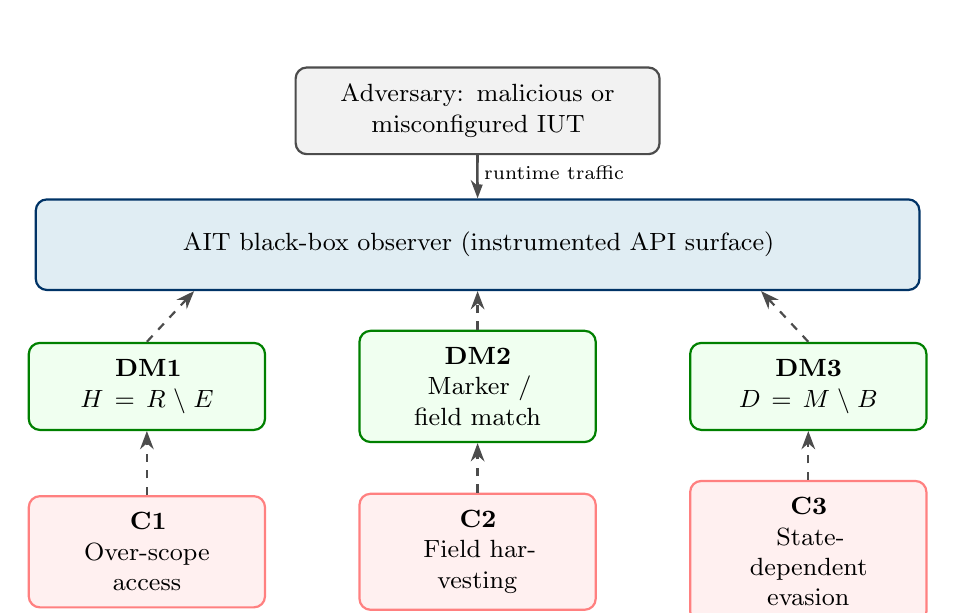
\begin{tikzpicture}[
        font=\small,
        capcol/.style={threatcap, minimum width=3.0cm},
        dmcol/.style={dmbox, minimum width=3.0cm}
    ]
        \node[svcbox, text width=4.2cm] (iut) at (0, 4.6)
            {Adversary: malicious or\\misconfigured IUT};
        \node[aitobs, text width=10.8cm, minimum height=1.15cm] (obs) at (0, 2.9)
            {AIT black-box observer (instrumented API surface)};
        \node[dmcol] (d1) at (-4.2, 1.1) {\textbf{DM1}\\$H = R \setminus E$};
        \node[dmcol] (d2) at (0, 1.1) {\textbf{DM2}\\Marker /\\field match};
        \node[dmcol] (d3) at (4.2, 1.1) {\textbf{DM3}\\$D = M \setminus B$};
        \node[capcol] (c1) at (-4.2, -1.0) {\textbf{C1}\\Over-scope\\access};
        \node[capcol] (c2) at (0, -1.0) {\textbf{C2}\\Field har-\\vesting};
        \node[capcol] (c3) at (4.2, -1.0) {\textbf{C3}\\State-\\dependent\\evasion};
        \draw[arrow] (iut) -- node[edgelbl, right, pos=0.4] {runtime traffic} (obs);
        \draw[arrow, dashed] (c1) -- (d1);
        \draw[arrow, dashed] (c2) -- (d2);
        \draw[arrow, dashed] (c3) -- (d3);
        \draw[arrow, dashed] (d1.north) -- ([xshift=-3.6cm]obs.south);
        \draw[arrow, dashed] (d2.north) -- (obs.south);
        \draw[arrow, dashed] (d3.north) -- ([xshift=3.6cm]obs.south);
    \end{tikzpicture}
    \caption{Threat capabilities (C1--C3) mapped to AIT detection mechanisms (DM1--DM3).
             Live allow/deny expectation checks remain future work / out of scope.}
    \label{fig:threat-map}
\end{figure}

\section{Research Contributions}

\begin{itemize}
    \item An integration-centric adversarial testing methodology treating the integration as the test subject, combining differential API fuzzing with taint-seeded data tracking.
    \item The AIT framework: a modular, open-source Coordinator API, Mock SaaS service, and Analysis Engine, detecting three violation categories with structured risk scoring.
    \item A dual-phase execution model (baseline / mutated) that surfaces state-dependent evasion (C3) invisible to static analysis and single-phase testing.
    \item An instrumentation-free taint-injection mechanism operating at the data layer, enabling precise run-attributed detection of sensitive field access.
    \item A live SaaS evaluation pipeline (\texttt{ait/live\_runner.py}) for instrumented sandbox probes; GitHub/Notion Task~6 empirical results remain \texttt{NOT RUN}/\textbf{BLOCKED} without credentials.
    \item A log-based replay experiment applying AIT's detection logic to researcher-constructed traces from public disclosures.
    \item A false negative analysis characterising four evasion scenarios that defeat the current detection model.
    \item A risk scoring sensitivity analysis over $\pm 30\%$ weight perturbation with band transitions recorded in offline artifacts.
    \item A multi-ecosystem mock evaluation harness with YAML-defined platform-inspired scenarios spanning Slack-, GitHub-, Gmail-, Notion-, and Trello-style REST idioms, with automated aggregation for reproducible tabular results.
    \item A read-only GitHub REST smoke probe plan (empirical rows \texttt{NOT RUN} without credentials), robustness/evasion YAML suites, and a micro-benchmark of Analysis Engine latency versus synthetic log width (generated timings).
\end{itemize}

\section{Novelty and Positioning}

Unlike prior API-testing and OAuth-auditing tools, AIT introduces an explicit verification axis:
integration-policy conformance --- do runtime calls and returned fields stay within an operational
policy artifact (\texttt{TargetConfig})? This axis is orthogonal to server-side vulnerability
discovery and to static OAuth auditing without behavioural reconciliation; AIT is a
policy-reconciliation framework deployed alongside --- not as a replacement for --- existing
fuzzers and permission tools.

% ══════════════════════════════════════════════════════════════════════════════
\chapter{Literature Survey}

\section{OAuth 2.0 Security and Permission Models}

OAuth 2.0 \cite{rfc6749} defines four grant types; the authorisation code flow with PKCE
\cite{rfc7636} predominates for third-party SaaS integrations. OpenID Connect \cite{oidc2014}
extends OAuth 2.0 for identity assertions.

Security research has focused on implementation vulnerabilities: Fett et al.\ \cite{fett2017}
identified redirect URI and token binding attacks; Felt et al.\ \cite{felt2012} showed users
misunderstand scope descriptions. The OWASP API Security Top 10 (2023) \cite{owaspapi2023}
identifies Broken Object Level Authorisation (BOLA) and Broken Function Level Authorisation
(BFLA) as leading API risks, both manifesting through over-privileged integrations.

Recent work addresses the enforcement gap directly. Mainka et al.\ \cite{mainka2022} showed
that OAuth scope validation is inconsistent across SaaS providers. De Carne de Carnavalet and
van Oorschot \cite{decarne2023} found systematic over-provisioning at scale across major
identity providers. Boucher et al.\ \cite{boucher2024} proposed static policy enforcement for
SaaS integration permission graphs but evaluated only declared configurations, not runtime
behaviour --- the gap AIT addresses. Lundberg et al.\ \cite{lundberg2024} proposed a runtime
OAuth scope enforcement proxy but require server-side middleware deployment, limiting
applicability to integrations without source access.

\section{API Fuzzing and Differential Testing}

AFL \cite{afl} and Boofuzz \cite{boofuzz} provide foundational coverage-guided and protocol
fuzzing. RESTler \cite{restler2019} introduced stateful REST fuzzing with producer-consumer
dependency sequencing. EvoMaster \cite{evomaster2019} applies evolutionary algorithms to
OpenAPI test generation. Atlidakis et al.\ \cite{atlidakis2020} extended RESTler with
property-based security checking rules.

Differential fuzzing --- comparing behaviour across configurations for the same inputs --- has
been applied to compilers \cite{yang2011} and cryptographic libraries \cite{petsios2017}.
Kim et al.\ \cite{kim2022} applied it to microservice API consistency checking. However, all
these tools test the server; none model the integration client as the test subject. AIT inverts
this perspective.

Benamara et al.\ \cite{benamara2020} introduced differential fuzzing for DPI evasion in QUIC,
demonstrating the applicability of differential approaches to protocol-layer behavioural
divergence. Bulekov et al.\ \cite{bulekov2023} introduced coverage-guided taint-directed web
API fuzzing, though requiring server-side instrumentation --- a constraint AIT explicitly
relaxes.

\section{Taint Analysis}

Static taint analysis \cite{livshits2005} identifies data flows without execution. Dynamic taint
analysis \cite{clause2007}, exemplified by TaintDroid \cite{taintdroid2014}, instruments
programs at runtime. Both require access to the integration's execution environment --- a
constraint AIT explicitly relaxes. Pan et al.\ \cite{pan2022} proposed privacy-preserving
synthetic data for API testing, a principle AIT operationalises through its taint-injection
mechanism.

\section{SaaS Security Auditing and Zero-Trust}

Commercial tools (Nudge Security, Grip Security, DoControl) provide OAuth grant visibility but
cannot observe runtime behaviour. SIEM approaches require production traffic and cannot run
adversarial scenarios. NIST SP 800-207 \cite{nist800207} formalises zero-trust, advocating
continuous workload verification; existing implementations address network-layer enforcement,
not API-behavioural conformance. Ding et al.\ \cite{ding2023} proposed continuous
authorisation under zero-trust but acknowledged absence of runtime behavioural testing tools.
Wermke et al.\ \cite{wermke2022} found developers rarely audit integration behaviour against
declared scopes post-deployment. Chandramouli \cite{chandramouli2023} surveys SaaS Security
Posture Management (SSPM) frameworks and identifies runtime behavioural verification as an
open research gap.

\section{Tool Capability Taxonomy}

Table~\ref{tab:tool-taxonomy} maps existing tools to capability dimensions. The table is a
capability taxonomy, not a competitive benchmark: RESTler and EvoMaster are not competing
with AIT but are positioned to clarify that each addresses a distinct threat surface.

\begin{table}[H]
    \centering
    \caption{Tool Capability Taxonomy (Adjacent Problem Spaces)}
    \label{tab:tool-taxonomy}
    \begin{tabularx}{\textwidth}{lXXXX}
        \toprule
        \textbf{Tool / Approach}  & \textbf{Scope Audit} & \textbf{Runtime Test} & \textbf{Diff.\ Phase} & \textbf{Taint} \\
        \midrule
        OAuth Audit Tools         & \checkmark           & ---                   & ---                   & ---            \\[4pt]
        RESTler \cite{restler2019}& ---                  & \checkmark            & ---                   & ---            \\[4pt]
        EvoMaster \cite{evomaster2019}& ---              & \checkmark            & ---                   & ---            \\[4pt]
        SIEM / Log Analysis       & Partial              & Reactive              & ---                   & ---            \\[4pt]
        TaintDroid$^\dagger$ \cite{taintdroid2014}& ---  & \checkmark            & ---                   & \checkmark     \\[4pt]
        Boucher et al.\ \cite{boucher2024}& \checkmark   & ---                   & ---                   & ---            \\[4pt]
        Lundberg et al.\ \cite{lundberg2024}& \checkmark & \checkmark            & ---                   & ---            \\[4pt]
        \textbf{AIT (Ours)}       & \checkmark           & \checkmark            & \checkmark            & \checkmark     \\
        \bottomrule
        \multicolumn{5}{l}{\footnotesize $^\dagger$Requires device/server instrumentation.}
    \end{tabularx}
\end{table}

\section{Summary of Research Gaps}

The survey reveals a clear gap: no existing tool simultaneously performs scope-level auditing,
runtime behavioural testing, differential phase comparison, and instrumentation-free taint
tracking against an operational policy artifact. Static OAuth auditors \cite{boucher2024} see
declared scopes but not traffic. Server-side fuzzers \cite{restler2019,evomaster2019} generate
server vulnerabilities but treat the integration as benign. Taint frameworks \cite{taintdroid2014}
require deep instrumentation access. AIT occupies the intersection that none of these tools cover,
establishing integration-policy conformance as a first-class, runtime-verifiable security property
(Figure~\ref{fig:positioning}).

\begin{figure}[H]
    \centering
    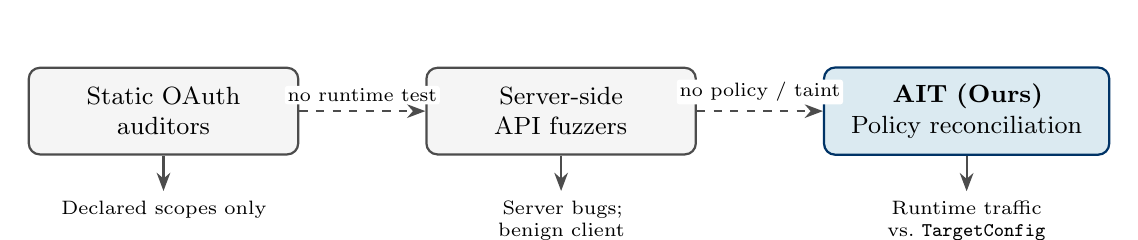
\begin{tikzpicture}[node distance=0.5cm and 1.6cm, font=\small]
        \node[gapother, text width=3.0cm] (static) {Static OAuth\\auditors};
        \node[gapother, text width=3.0cm, right=of static] (fuzz) {Server-side\\API fuzzers};
        \node[gapait, text width=3.2cm, right=of fuzz] (ait) {\textbf{AIT (Ours)}\\Policy reconciliation};
        \node[below=0.45cm of static, font=\scriptsize, text width=3.0cm, align=center] (s1)
            {Declared scopes only};
        \node[below=0.45cm of fuzz, font=\scriptsize, text width=3.0cm, align=center] (f1)
            {Server bugs; benign client};
        \node[below=0.45cm of ait, font=\scriptsize, text width=3.2cm, align=center] (a1)
            {Runtime traffic vs.\ \texttt{TargetConfig}};
        \draw[arrow] (static) -- (s1);
        \draw[arrow] (fuzz) -- (f1);
        \draw[arrow] (ait) -- (a1);
        \draw[arrow, dashed] (static.east) --
            node[edgelbl, above=2pt, midway, fill=white, inner sep=1pt] {no runtime test}
            (fuzz.west);
        \draw[arrow, dashed] (fuzz.east) --
            node[edgelbl, above=2pt, midway, fill=white, inner sep=1pt] {no policy / taint}
            (ait.west);
    \end{tikzpicture}

    \vspace{0.6em}
    {\footnotesize
    \renewcommand{\arraystretch}{1.2}
    \begin{tabular}{lccc}
        \toprule
        \textbf{Capability} & \textbf{Static} & \textbf{Fuzz} & \textbf{AIT} \\
        \midrule
        Scope audit        & \checkmark      & ---           & \checkmark \\
        Runtime test       & ---             & \checkmark    & \checkmark \\
        Diff.\ phase       & ---             & ---           & \checkmark \\
        Taint (no instr.)  & ---             & ---           & \checkmark \\
        \bottomrule
    \end{tabular}
    }
    \caption{Positioning of AIT relative to adjacent tool classes. Dashed arrows highlight
             capability gaps between tool classes; the table shows which dimensions each class
             covers (cf.\ Table~\ref{tab:tool-taxonomy}).}
    \label{fig:positioning}
\end{figure}

% ══════════════════════════════════════════════════════════════════════════════
\chapter{System Design}
\label{ch:design}

\section{High-Level Architecture}

AIT comprises three independently deployable microservices communicating over HTTP: the
\textbf{Coordinator API} (orchestration), the \textbf{Mock SaaS Service} (instrumented target
simulator), and the \textbf{Integration Under Test (IUT)}. A separate Live SaaS Runner
(\texttt{ait/live\_runner.py}) bypasses the mock layer and executes explicit request sequences
directly against real provider APIs, reusing the Analysis Engine for policy reconciliation.

\begin{figure}[H]
    \centering
    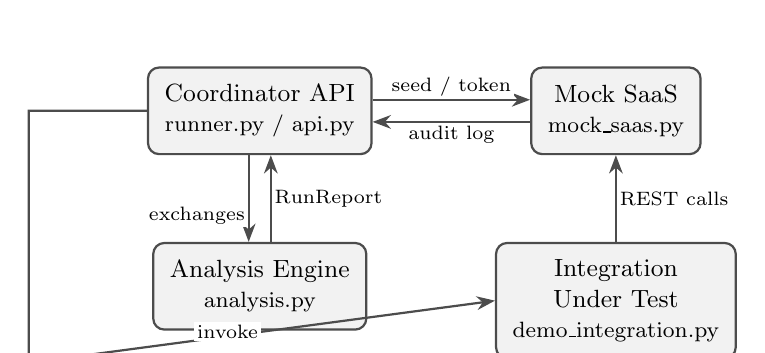
\begin{tikzpicture}[
        node distance=1.1cm and 2.0cm
    ]
        \node[svcbox] (coord)
            {Coordinator API\\
            {\footnotesize runner.py / api.py}};
        \node[svcbox, right=of coord] (mock)
            {Mock SaaS\\
            {\footnotesize mock\_saas.py}};
        \node[svcbox, below=of mock] (iut)
            {Integration\\
            Under Test\\
            {\footnotesize demo\_integration.py}};
        \node[svcbox, below=of coord] (ae)
            {Analysis Engine\\
            {\footnotesize analysis.py}};
        \draw[arrow]
            ([yshift=4pt]coord.east) --
            node[above, font=\scriptsize, fill=white, inner sep=1pt]
            {seed / token}
            ([yshift=4pt]mock.west);
        \draw[arrow]
            ([yshift=-4pt]mock.west) --
            node[below, font=\scriptsize, fill=white, inner sep=1pt]
            {audit log}
            ([yshift=-4pt]coord.east);
        \draw[arrow]
            (coord.west)
            -- ++(-1.5,0)
            -- ++(0,-3.2)
            -- node[pos=0.5, left, font=\scriptsize, fill=white, inner sep=1pt] {invoke}
            (iut.west);
        \draw[arrow]
            (iut.north)
            -- node[right, font=\scriptsize, fill=white, inner sep=1pt]
            {REST calls}
            (mock.south);
        \draw[arrow]
            ([xshift=-4pt]coord.south) --
            node[pos=0.7, left, font=\scriptsize, fill=white, inner sep=1pt]
            {exchanges}
            ([xshift=-4pt]ae.north);
        \draw[arrow]
            ([xshift=4pt]ae.north) --
            node[right, font=\scriptsize, fill=white, inner sep=1pt]
            {RunReport}
            ([xshift=4pt]coord.south);
    \end{tikzpicture}
    \caption{AIT system architecture showing data flow between the Coordinator API, Mock SaaS
             Service, Integration Under Test, and Analysis Engine.}
    \label{fig:arch}
\end{figure}

\section{Coordinator API}

The Coordinator exposes \texttt{POST /runs} and \texttt{GET /runs/\{run\_id\}}. On invocation
it: generates a unique 12-character hexadecimal \texttt{run\_id}; resolves an OAuth token; seeds
the Mock SaaS with taint data; invokes the IUT under baseline and mutated conditions; retrieves
the audit log; and forwards exchanges to the Analysis Engine.

\texttt{TargetConfig} objects encode the security policy: \texttt{expected\_endpoints},
\texttt{expected\_scopes}, and \texttt{sensitive\_markers}. Figure~\ref{fig:pipeline} shows the
end-to-end detection pipeline.

\begin{figure}[H]
    \centering
    \resizebox{\textwidth}{!}{%
    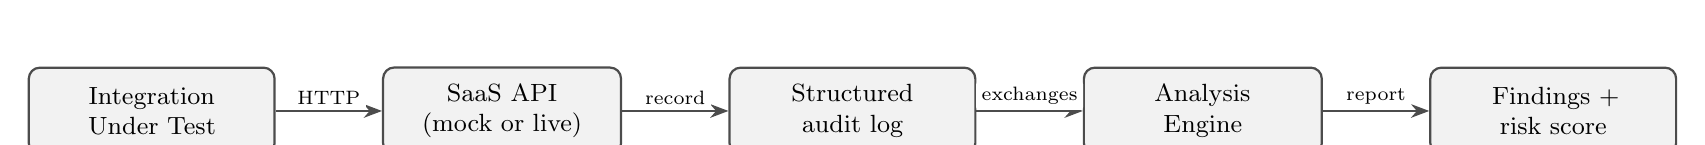
\begin{tikzpicture}[node distance=0.5cm and 1.35cm]
        \node[svcbox, text width=2.7cm] (iut) {Integration\\Under Test};
        \node[svcbox, right=of iut, text width=2.6cm] (api) {SaaS API\\(mock or live)};
        \node[svcbox, right=of api, text width=2.7cm] (log) {Structured\\audit log};
        \node[svcbox, right=of log, text width=2.6cm] (ae) {Analysis\\Engine};
        \node[svcbox, right=of ae, text width=2.7cm] (rep) {Findings +\\risk score};
        \draw[arrow] (iut) -- node[edgelbl, above, midway] {HTTP} (api);
        \draw[arrow] (api) -- node[edgelbl, above, midway] {record} (log);
        \draw[arrow] (log) -- node[edgelbl, above, midway] {exchanges} (ae);
        \draw[arrow] (ae) -- node[edgelbl, above, midway] {report} (rep);
    \end{tikzpicture}%
    }
    \caption{End-to-end detection pipeline: observed integration traffic is normalised into
             \texttt{CapturedExchange} records, analysed against policy, and emitted as
             structured findings. The same pipeline is used for both mock and live evaluations.}
    \label{fig:pipeline}
\end{figure}

\section{Mock SaaS Service}

The Mock SaaS retains the original CRM surface (\texttt{/api/v1/customers},
\texttt{/customers/\{id\}}, \texttt{/customers/\{id\}/notes},
\texttt{/customers/\{id\}/billing}) for mechanism-isolation experiments. The billing endpoint is
omitted from \texttt{expected\_endpoints} but accessible via the over-provisioned scope,
instantiating capabilities C1 and C2. Administrative routes (\texttt{/oauth/token},
\texttt{/admin/seed}, \texttt{/admin/audit/\{run\_id\}}) support the Coordinator. The service
also exposes platform-inspired REST paths patterned after Slack, GitHub, Google Gmail, Notion,
and Trello, so DM1--DM3 operate uniformly across both the CRM corpus and the extended corpus.

\section{Live SaaS Runner}

The \texttt{ait/live\_runner.py} module implements a direct evaluation path for explicit sandbox
scenarios. It reads bearer tokens from environment variables, executes operator-defined baseline
and mutated requests against real SaaS APIs (e.g., \texttt{api.github.com},
\texttt{api.notion.com}), converts HTTP responses into \texttt{CapturedExchange} records
without mock-side instrumentation, and adds policy findings when a request expected to be denied
succeeds or vice versa.

\section{Analysis Engine and Data Model}

The Analysis Engine applies four detection mechanisms to \texttt{CapturedExchange} objects and
produces a \texttt{RunReport} with \texttt{Finding} objects and a risk score. All data is typed
via Pydantic v2 models, enabling deterministic JSON serialisation and downstream SIEM ingestion.

\section{CI/CD Deployment Sketch}

A practical deployment pattern runs AIT from CI/CD before shipping an integration change:
failures gate merges when new endpoints or sensitive markers appear relative to the checked-in
policy YAML.

\begin{figure}[H]
    \centering
    \resizebox{\textwidth}{!}{%
    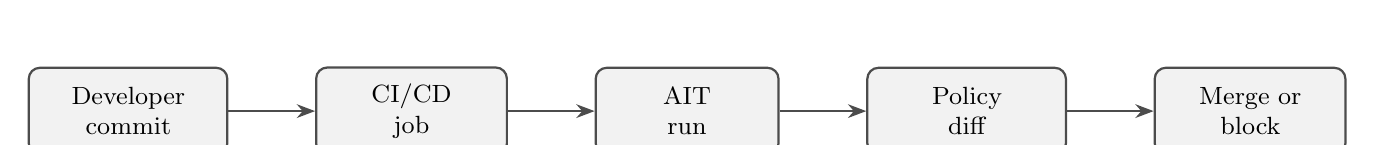
\begin{tikzpicture}[node distance=0.4cm and 1.1cm, font=\small]
        \node[svcbox, text width=2.1cm] (dev) {Developer\\commit};
        \node[svcbox, right=of dev, text width=2.0cm] (cicd) {CI/CD\\job};
        \node[svcbox, right=of cicd, text width=1.9cm] (ait) {AIT\\run};
        \node[svcbox, right=of ait, text width=2.1cm] (pol) {Policy\\diff};
        \node[svcbox, right=of pol, text width=2.0cm] (gate) {Merge or\\block};
        \draw[arrow] (dev) -- (cicd);
        \draw[arrow] (cicd) -- (ait);
        \draw[arrow] (ait) -- (pol);
        \draw[arrow] (pol) -- (gate);
    \end{tikzpicture}%
    }
    \caption{Deployment sketch: integration changes are gated on AIT policy reconciliation
             before release.}
    \label{fig:cicd}
\end{figure}

% ══════════════════════════════════════════════════════════════════════════════
\chapter{Methodology}

\section{Dual-Phase Execution Model}

Figure~\ref{fig:dualphase} illustrates the dual-phase flow, designed to address adversary
capability C3. Two execution phases differ only in the state signal sent to the IUT:

\begin{figure}[H]
    \centering
    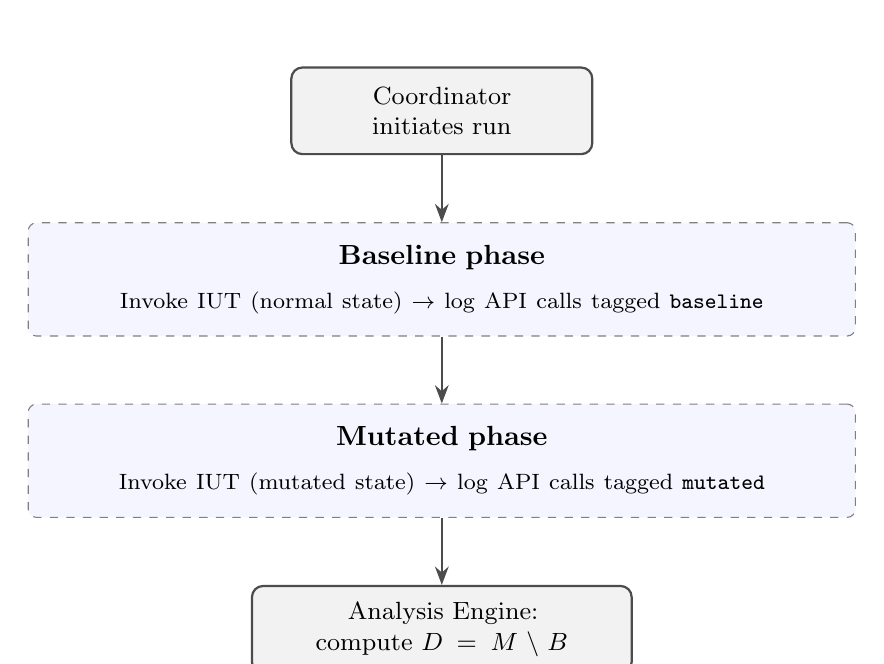
\begin{tikzpicture}[node distance=0.85cm, every node/.style={align=center}]
        \node[svcbox, text width=3.4cm] (start) {Coordinator\\initiates run};
        \node[phase, below=of start, text width=0.82\textwidth, minimum height=1.35cm] (bp) {%
            \textbf{Baseline phase}\\[4pt]
            \footnotesize Invoke IUT (normal state)
            $\rightarrow$ log API calls tagged \texttt{baseline}%
        };
        \node[phase, below=of bp, text width=0.82\textwidth, minimum height=1.35cm] (mp) {%
            \textbf{Mutated phase}\\[4pt]
            \footnotesize Invoke IUT (mutated state)
            $\rightarrow$ log API calls tagged \texttt{mutated}%
        };
        \node[svcbox, below=of mp, text width=4.4cm] (ae2) {%
            Analysis Engine:\\compute $D = M \setminus B$%
        };
        \draw[arrow] (start) -- (bp);
        \draw[arrow] (bp) -- (mp);
        \draw[arrow] (mp) -- (ae2);
    \end{tikzpicture}
    \caption{Dual-phase execution. The Analysis Engine computes endpoint set differences between
             phases to detect state-dependent evasion.}
    \label{fig:dualphase}
\end{figure}

\begin{itemize}
    \item \textbf{Baseline Phase:} Integration invoked under normal state; all API calls recorded with label \texttt{"baseline"}.
    \item \textbf{Mutated Phase:} Integration invoked with \texttt{phase="mutated"}, activating feature flags or latent branches; calls recorded with label \texttt{"mutated"}.
\end{itemize}

Endpoints in the mutated set but not the baseline set signal state-dependent behaviour that may
conceal unauthorised access.

\section{Taint-Seeded Data Tracking}

Before each run, \texttt{POST /admin/seed} updates sensitive fields in Mock SaaS records
with run-specific synthetic tokens (e.g., \texttt{billing\_email = \{run\_id\}@example.test}).
These values are globally unique, contain no real user data, and serve two roles:

\begin{itemize}
    \item \textbf{Taint injection:} Enabling response-level detection of sensitive field access.
    \item \textbf{Run attribution:} Ensuring concurrent test runs cannot contaminate one another's audit records.
\end{itemize}

No IUT instrumentation is required. In the live SaaS runner, sensitive markers are checked
against actual API response payloads; real credentials or PII in responses are never logged in
plaintext.

\section{Detection Mechanisms}

\textbf{DM1 --- Hidden Endpoint Detection (addresses C1):}
\[
    H = R \setminus E
\]
where $R$ = reached endpoints, $E$ = expected endpoints. Each $h \in H$ yields a
HIGH-severity \texttt{HIDDEN\_ENDPOINT} finding.

\textbf{DM2 --- Sensitive Field Access Detection (addresses C2):}
Any \texttt{CapturedExchange} where \texttt{contains\_sensitive\_marker} is true or response
fields intersect \texttt{sensitive\_markers} yields a CRITICAL-severity
\texttt{SENSITIVE\_FIELD\_ACCESS} finding.

\textbf{DM3 --- Behavioural Divergence Detection (addresses C3):}
\[
    D = M \setminus B
\]
where $M$ = mutated-phase endpoint set, $B$ = baseline-phase endpoint set. Non-empty $D$
yields a HIGH-severity \texttt{BEHAVIORAL\_DIVERGENCE} finding.

Allow/deny expectation checks against live HTTP status codes are out of scope for the
current release (future work / not yet implemented); the live runner reuses DM1--DM3 on
captured exchanges only.
Figure~\ref{fig:dm-map} consolidates the mapping from threat classes to detectors and severities.

\begin{figure}[H]
    \centering
    {\footnotesize
    \renewcommand{\arraystretch}{1.35}
    \setlength{\tabcolsep}{6pt}
    \begin{tabular}{@{}>{\raggedright\arraybackslash}p{2.35cm}
                         >{\raggedright\arraybackslash}p{2.65cm}
                         >{\raggedright\arraybackslash}p{3.05cm}
                         >{\raggedright\arraybackslash}p{1.85cm}@{}}
        \toprule
        \textbf{Threat} & \textbf{Detector} & \textbf{Finding} & \textbf{Severity} \\
        \midrule
        C1 over-scope &
            DM1: $H = R \setminus E$ &
            \texttt{HIDDEN\_ENDPOINT} &
            HIGH \\
        C2 field harvest &
            DM2: markers &
            \texttt{SENSITIVE\_FIELD\_ACCESS} &
            CRITICAL \\
        C3 evasion &
            DM3: $D = M \setminus B$ &
            \texttt{BEHAVIORAL\_DIVERGENCE} &
            HIGH \\
        \bottomrule
    \end{tabular}
    }
    \caption{Detection mechanism map: each adversary capability class maps to a detector, finding
             category, and default severity band used in risk scoring.}
    \label{fig:dm-map}
\end{figure}

\section{Informal Detection Guarantees}

Under black-box observation of traffic recorded in the audit log and relative to a supplied
\texttt{TargetConfig}, AIT reports: (G1) any reached path outside \texttt{expected\_endpoints};
(G2) responses whose extracted fields intersect \texttt{sensitive\_markers} or carry the
synthetic taint flag; and (G3) phase-specific endpoint-set differences consistent with DM3.
These are sound with respect to the observed run --- they do not prove absence
of violations outside the logged surface.

\section{Risk Scoring Model}

\[
    S = \min\!\bigl(100,\; w_H \cdot |H| + w_F \cdot |F_s| + w_D \cdot |D|\bigr)
\]

Weights $(w_H, w_F, w_D) = (25, 20, 15)$ are heuristic design constants inspired by the
CVSS v3.1 severity taxonomy
\cite{cvss31} (not empirically calibrated scores): C1 maps to Scope:Changed/Confidentiality:High (base score 7.5--9.0, $w_H=25$);
C2 maps to Confidentiality:High without scope change (6.5--7.5, $w_F=20$); C3 represents
architectural risk without confirmed data access (4.0--6.0, $w_D=15$). Score bands: 0--25
(Low), 26--50 (Medium), 51--75 (High), 76--100 (Critical).
Figure~\ref{fig:risk-bands} shows the score bands used for triage.

\begin{figure}[H]
    \centering
    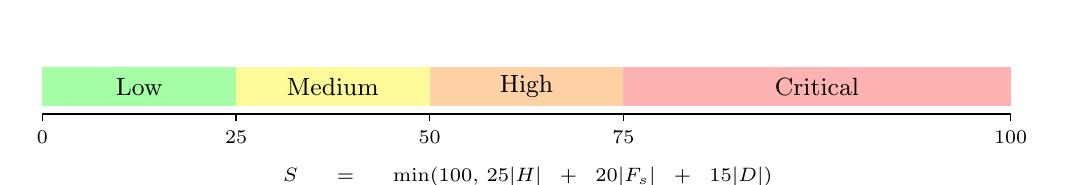
\begin{tikzpicture}[x=0.078\textwidth, y=0.7cm, font=\small]
        \draw[thick] (0,0) -- (13,0);
        \foreach \x/\lbl in {0/0, 2.6/25, 5.2/50, 7.8/75, 13/100} {
            \draw (\x,0) -- (\x,-0.12) node[below, font=\scriptsize] {\lbl};
        }
        \fill[green!35]  (0,0.15) rectangle (2.6,0.85);
        \fill[yellow!40] (2.6,0.15) rectangle (5.2,0.85);
        \fill[orange!35] (5.2,0.15) rectangle (7.8,0.85);
        \fill[red!30]    (7.8,0.15) rectangle (13,0.85);
        \node at (1.3,0.5) {Low};
        \node at (3.9,0.5) {Medium};
        \node at (6.5,0.5) {High};
        \node at (10.4,0.5) {Critical};
        \node[below=0.55cm, font=\scriptsize, text width=12cm, align=center] at (6.5,0) {%
            $S = \min(100,\, 25|H| + 20|F_s| + 15|D|)$%
        };
    \end{tikzpicture}
    \caption{Risk score bands for aggregate triage. Scenario~S3 (one hidden endpoint, two
             sensitive fields, one divergence) yields $S=80$ (Critical) under base weights.}
    \label{fig:risk-bands}
\end{figure}

% ══════════════════════════════════════════════════════════════════════════════
\chapter{Hardware and Software Requirements}
\label{ch:hwsw}

This chapter specifies the minimum and recommended hardware configurations and the complete
software stack required to deploy, develop, and evaluate the AIT framework.

\section{Hardware Requirements}

AIT is a lightweight Python-based framework designed to run on commodity developer hardware.
No specialised hardware is required for the proof-of-concept deployment; the following
specifications reflect the configurations used during development and evaluation.

\begin{table}[H]
    \centering
    \caption{Hardware Requirements}
    \label{tab:hardware}
    \begin{tabularx}{\textwidth}{lXX}
        \toprule
        \textbf{Component} & \textbf{Minimum} & \textbf{Recommended} \\
        \midrule
        CPU       & Dual-core, 2.0 GHz      & Quad-core, 2.5 GHz or faster         \\[4pt]
        RAM       & 4 GB                    & 8 GB or more                          \\[4pt]
        Storage   & 5 GB free disk space    & 20 GB SSD (for logs and result artifacts) \\[4pt]
        Network   & Broadband internet      & Low-latency connection ($<$50 ms RTT to provider APIs) \\[4pt]
        OS        & 64-bit Linux, macOS, or Windows 10/11 & Ubuntu 22.04 LTS or macOS 14+ \\
        \bottomrule
    \end{tabularx}
\end{table}

\textbf{Notes on hardware context:}

\begin{itemize}
    \item Offline mock assessments are dominated by in-process ASGI transport rather than Analysis Engine compute; see generated benchmark timings for measured medians.
    \item Live SaaS assessments (GitHub, Notion sandbox runs) are \texttt{NOT RUN} without credentials; measured WAN timings are therefore unavailable.
    \item Analysis Engine micro-benchmark rows are regenerated from the hashed offline artifact (Table~\ref{tab:benchmark}); do not cite hand-copied latencies.
    \item A production deployment with persistent storage (PostgreSQL or Redis backend) will require higher RAM and I/O throughput than the minimum specification.
\end{itemize}

\section{Software Requirements}

\subsection{Core Runtime}

\begin{table}[H]
    \centering
    \caption{Core Software Stack}
    \label{tab:tech-stack}
    \begin{tabular}{lll}
        \toprule
        \textbf{Component}         & \textbf{Technology / Version}          & \textbf{Role}                    \\
        \midrule
        Language Runtime           & Python 3.11+                           & Primary runtime                  \\[4pt]
        Web Framework              & FastAPI (0.100+)                       & Coordinator API and Mock SaaS    \\[4pt]
        ASGI Server                & Uvicorn (0.23+)                        & HTTP serving                     \\[4pt]
        HTTP Client                & asyncio / httpx (0.24+)                & Async outbound requests          \\[4pt]
        Data Validation            & Pydantic v2 (2.0+)                     & Type-safe data models            \\[4pt]
        Policy Definitions         & PyYAML (6.0+)                          & YAML scenario parsing            \\[4pt]
        Package Manager            & pip / venv or conda                    & Dependency management            \\
        \bottomrule
    \end{tabular}
\end{table}

\subsection{Development and Testing Tools}

\begin{table}[H]
    \centering
    \caption{Development and Testing Tools}
    \label{tab:dev-tools}
    \begin{tabular}{lll}
        \toprule
        \textbf{Tool}              & \textbf{Version}     & \textbf{Purpose}                         \\
        \midrule
        pytest                     & 7.0+                 & Unit and integration test runner          \\[4pt]
        pytest-asyncio             & 0.21+                & Async test support                        \\[4pt]
        httpx (test client)        & 0.24+                & ASGI transport for in-process testing     \\[4pt]
        python-dotenv              & 1.0+                 & Environment variable management           \\[4pt]
        PyYAML                     & 6.0+                 & YAML scenario loading                     \\[4pt]
        Git                        & 2.x                  & Version control for YAML policies         \\[4pt]
        Docker (optional)          & 24.x+                & Containerised deployment                  \\
        \bottomrule
    \end{tabular}
\end{table}

\subsection{Network and API Access}

\begin{table}[H]
    \centering
    \caption{Network and API Access Requirements}
    \label{tab:network}
    \begin{tabular}{lp{9cm}}
        \toprule
        \textbf{Requirement}           & \textbf{Details}                                                          \\
        \midrule
        Localhost ports                & 8000 (Coordinator API), 8001 (Mock SaaS), 8002 (Integration Under Test)  \\[4pt]
        Internet access                & Required for live SaaS evaluation (GitHub, Notion, Slack, Google APIs)   \\[4pt]
        OAuth / PAT tokens             & Read-only personal access tokens for sandbox accounts; stored in environment variables, never committed to version control \\[4pt]
        Rate limit awareness           & Production deployments must implement exponential backoff and respect \texttt{Retry-After} headers from provider APIs \\[4pt]
        Firewall / proxy rules         & Outbound HTTPS (port 443) to \texttt{api.github.com}, \texttt{api.notion.com} and other provider endpoints \\
        \bottomrule
    \end{tabular}
\end{table}

\subsection{Optional Production Dependencies}

For production-grade or concurrent deployment, the following additional components are required
to replace the in-memory state store:

\begin{table}[H]
    \centering
    \caption{Optional Production Dependencies}
    \label{tab:prod-deps}
    \begin{tabular}{lll}
        \toprule
        \textbf{Component}     & \textbf{Technology}      & \textbf{Purpose}                         \\
        \midrule
        Persistent store       & PostgreSQL 15+ or Redis 7+  & Replace in-memory run/audit log store  \\[4pt]
        Container runtime      & Docker / Kubernetes         & Microservice isolation and scaling     \\[4pt]
        CI/CD integration      & GitHub Actions / Jenkins    & Automated policy regression gate       \\[4pt]
        SIEM connector         & Splunk, Elastic, or custom  & Downstream ingestion of JSON findings  \\
        \bottomrule
    \end{tabular}
\end{table}

\subsection{Installation and Setup}

A standard development environment is set up as follows:

\begin{lstlisting}[
    style=pythonstyle,
    caption={Environment setup commands},
    label={lst:setup}
]
# Clone the repository
git clone https://github.com/<org>/ait.git && cd ait

# Create and activate a virtual environment
python3 -m venv .venv
source .venv/bin/activate          # Linux / macOS
# .venv\Scripts\activate           # Windows

# Install all dependencies
pip install -r requirements.txt

# Set live SaaS tokens (never commit these)
export AIT_GITHUB_TOKEN="ghp_xxxxxxxxxxxx"
export AIT_NOTION_TOKEN="secret_xxxxxxxxxxxx"

# Start all three services in separate terminals
uvicorn coordinator.api:app --port 8000
uvicorn mock_saas.app:app  --port 8001
uvicorn iut.demo_integration:app --port 8002

# Run the full mock paper-results pipeline
python generate_paper_results.py

# Run live SaaS evaluation
python generate_live_saas_results.py
\end{lstlisting}

\subsection{Implementation: Core Detection Logic}

The following listing shows the core Analysis Engine implementing DM1--DM3 using Pydantic v2
data models. This code runs on the software stack specified above.

\begin{lstlisting}[
    style=pythonstyle,
    caption={Core Analysis Engine detection logic (DM1, DM2, DM3).},
    label={lst:analysis-engine}
]
from pydantic import BaseModel
from typing import List, Set


class TargetConfig(BaseModel):
    expected_endpoints: List[str]
    expected_scopes: List[str]
    sensitive_markers: List[str]


class Finding(BaseModel):
    category: str   # HIDDEN_ENDPOINT | SENSITIVE_FIELD_ACCESS | BEHAVIORAL_DIVERGENCE
    severity: str   # CRITICAL | HIGH | MEDIUM | LOW
    detail: str


def analyze_run(
    exchanges: list,
    config: TargetConfig
) -> tuple[list[Finding], int]:
    """Apply DM1, DM2, DM3 to CapturedExchange records."""
    findings: list[Finding] = []

    reached: Set[str]  = {e.endpoint for e in exchanges}
    expected: Set[str] = set(config.expected_endpoints)
    baseline: Set[str] = {e.endpoint for e in exchanges if e.phase == "baseline"}
    mutated: Set[str]  = {e.endpoint for e in exchanges if e.phase == "mutated"}

    # DM1 -- Hidden Endpoint Detection
    for hidden in reached - expected:
        findings.append(Finding(
            category="HIDDEN_ENDPOINT",
            severity="HIGH",
            detail=f"Undeclared endpoint reached: {hidden}"
        ))

    # DM2 -- Sensitive Field Access Detection
    for exchange in exchanges:
        if exchange.contains_sensitive_marker:
            findings.append(Finding(
                category="SENSITIVE_FIELD_ACCESS",
                severity="CRITICAL",
                detail=f"Sensitive marker in response to {exchange.endpoint}"
            ))

    # DM3 -- Behavioural Divergence Detection
    for divergent in mutated - baseline:
        findings.append(Finding(
            category="BEHAVIORAL_DIVERGENCE",
            severity="HIGH",
            detail=f"Endpoint only reached in mutated phase: {divergent}"
        ))

    h = len([f for f in findings if f.category == "HIDDEN_ENDPOINT"])
    fs = len([f for f in findings if f.category == "SENSITIVE_FIELD_ACCESS"])
    d = len([f for f in findings if f.category == "BEHAVIORAL_DIVERGENCE"])
    score = min(100, 25 * h + 20 * fs + 15 * d)

    return findings, score
\end{lstlisting}

\begin{lstlisting}[
    style=pythonstyle,
    caption={Live SaaS runner sketch: allowlisted GETs and DM1--DM3 analysis (allow/deny expectation checks are future work).},
    label={lst:live-runner}
]
import os
import httpx
import yaml
from analysis import TargetConfig, analyze_run


def run_live_scenario(scenario_file: str) -> dict:
    """Execute a YAML-defined scenario against a live SaaS provider."""
    with open(scenario_file) as f:
        scenario = yaml.safe_load(f)

    token    = os.environ[scenario["token_env_var"]]
    base_url = scenario["base_url"]
    headers  = {"Authorization": f"Bearer {token}"}
    exchanges = []

    for request in scenario["requests"]:
        resp = httpx.get(f"{base_url}{request['path']}", headers=headers)
        exchanges.append({
            "path": request["path"],
            "status_code": resp.status_code,
            "phase": request.get("phase", "baseline"),
        })

    # Live path reuses DM1--DM3 via analyze_run; allow/deny checks are out of scope.
    report = analyze_run(scenario["id"], TargetConfig(**scenario["target"]), exchanges)
    return {"findings": report.findings, "risk_score": report.risk_score}
\end{lstlisting}

\subsection{Functional Requirements}

The following functional requirements translate the system's threat model and architectural
goals into concrete implementation behaviours.

\begin{longtable}{p{1.2cm}p{3.2cm}p{9.1cm}}
    \toprule
    \textbf{ID} & \textbf{Requirement} & \textbf{Description} \\
    \midrule
    \endhead
    FR-1 & TargetConfig Policy   &
        The system MUST accept a \texttt{TargetConfig} object defining
        \texttt{expected\_endpoints}, \texttt{expected\_scopes}, and
        \texttt{sensitive\_markers} for each integration run.                                  \\[6pt]
    FR-2 & YAML Policy Files     &
        Policies MUST be definable as version-controlled YAML files validated against the
        \texttt{TargetConfig} schema, enabling deterministic reproduction of all reported
        results.                                                                               \\[6pt]
    FR-3 & Run Isolation         &
        Each run MUST be assigned a unique 12-character hexadecimal \texttt{run\_id} for
        taint seeding and audit log attribution, ensuring concurrent runs cannot contaminate
        one another's records.                                                                 \\[6pt]
    FR-4 & Baseline Phase        &
        The Coordinator MUST invoke the IUT under normal state, recording all API calls
        with label \texttt{"baseline"}.                                                        \\[6pt]
    FR-5 & Mutated Phase         &
        The Coordinator MUST invoke the IUT with \texttt{phase="mutated"} to activate
        latent feature flags, recording all calls with label \texttt{"mutated"}.               \\[6pt]
    FR-6 & Divergence Detection  &
        The Analysis Engine MUST compute $D = M \setminus B$ and raise a
        \texttt{BEHAVIORAL\_DIVERGENCE} finding for each endpoint in $D$.                      \\[6pt]
    FR-7 & Hidden Endpoint (DM1) &
        The system MUST raise a HIGH-severity \texttt{HIDDEN\_ENDPOINT} finding for every
        endpoint reached that is absent from \texttt{expected\_endpoints}.                     \\[6pt]
    FR-8 & Sensitive Field (DM2) &
        The system MUST raise a CRITICAL-severity \texttt{SENSITIVE\_FIELD\_ACCESS} finding
        whenever a response contains a value matching \texttt{sensitive\_markers}.             \\[6pt]
    FR-9 & Structured Output    &
        The system MUST produce a structured JSON \texttt{RunReport} for SIEM ingestion
        and CI/CD gating.                                                                      \\[6pt]
    FR-10 & Risk Score           &
        The system MUST compute $S = \min(100,\,25|H|+20|F_s|+15|D|)$ and classify it
        into Low / Medium / High / Critical bands.                                             \\
    \bottomrule
    \caption{Functional Requirements}
    \label{tab:fr}
\end{longtable}

% ══════════════════════════════════════════════════════════════════════════════
\chapter{Experimental Evaluation}

\section{Evaluation Design and Scope}

The evaluation has five components:

\begin{itemize}
    \item \textbf{Controlled mock-environment experiments:} A 16-scenario offline corpus --- 6~CRM scenarios (3~isolation + 3~controls) and 10~platform-inspired mocks (7~violation-oriented + 3~compliant controls).
    \item \textbf{Live SaaS evaluation:} Executing explicit sandbox scenarios against real provider APIs (GitHub and Notion).
    \item \textbf{Read-only GitHub REST smoke probe:} Under an explicit allowlist policy.
    \item \textbf{Tool capability comparison:} With RESTler and EvoMaster.
    \item \textbf{Log-based replay:} Applying AIT's detection logic to researcher-constructed traces from public disclosures.
\end{itemize}

\section{Mock Environment: Test Scenarios}

Three scenarios isolate and combine detection mechanisms:

\begin{itemize}
    \item \textbf{S1 --- C1 only:} IUT accesses billing endpoint in both phases; no taint configured.
    \item \textbf{S2 --- C2 only:} IUT accesses only declared endpoints; responses contain tainted field values.
    \item \textbf{S3 --- C1 + C2 + C3 combined:} IUT accesses billing in the mutated phase only, with tainted \texttt{billing\_email} and \texttt{tax\_id}.
\end{itemize}

\section{Mock Environment: Detection Results}

% CLAIM:mock-overall-f1
% CLAIM:mock-category-metrics
Category precision/recall/F1 with TP/FP/FN denominators over the offline
mock corpus (regenerated from \texttt{scenario\_metrics}):

\begin{table}[H]
    \centering
    \caption{Detection Performance, Offline Mock Corpus (category metrics
    with micro-average; implementation validation under injected labels)}
    \label{tab:mock-results}
    \footnotesize
    \input{results/generated/mock_detection_results.tex}
\end{table}

Under injected labels, AIT's implementation matches the intended DM1--DM3 logic
on this controlled corpus. Perfect controlled scores, when observed, validate
implementation behaviour rather than broad effectiveness.

\section{Platform-Inspired Mock Suite}

% CLAIM:platform-scenario-risks
\begin{table}[H]
    \centering
    \caption{Platform-Inspired Mock Results (risk scores from offline
    scenario artifacts; synthetic mocks)}
    \label{tab:platform-results}
    \footnotesize
    \input{results/generated/platform_scenario_results.tex}
\end{table}

AIT maintains detection on heterogeneous platform-inspired mock idioms while
reporting zero risk on compliant baselines present in the generated table.

\section{Live SaaS Evaluation}

\begin{table}[H]
    \centering
    \caption{Live SaaS Evaluation Results (Sandbox Accounts;
    unavailable artifacts render as \texttt{NOT RUN})}
    \label{tab:live-results}
    \footnotesize
    \input{results/generated/live_results.tex}
\end{table}

Live sandbox Task~6 remains \textbf{BLOCKED} without credentials; rows above are
\texttt{NOT RUN}. The live runner design targets positive and negative control plans
on GitHub and Notion; empirical claims await redacted artifacts from real sandbox runs.

\section{Live GitHub REST Smoke Probe}

A separate read-only probe plan exercises \texttt{api.github.com} under a stricter policy
allowlisting only \texttt{/user}, with additional undeclared \texttt{/user/repos} and
\texttt{/user/orgs} requests. Empirical smoke-probe results remain \texttt{NOT RUN}
until a hashed live artifact is selected. When executed, the signal of interest is policy
mismatch relative to the allowlist, not server-side exploitability.

\section{Robustness and Noise}

% CLAIM:robustness-suite
% CLAIM:reproducibility-5
Robustness and evasion YAML cover noise, partial exposure, path ambiguity, FN4
field-alias negatives, and model-boundary cases. Table~\ref{tab:robust}
(\texttt{robustness\_results}) reports selected-artifact status from the offline
release gate. Deterministic reproducibility across five repetitions is recorded
in the hashed \texttt{reproducibility} artifact.

\begin{table}[H]
    \centering
    \caption{Robustness / Evasion Suite Status}
    \label{tab:robust}
    \input{results/generated/robustness_results.tex}
\end{table}

\section{Tool Capability Comparison}

Until a hashed \texttt{tool\_comparison} artifact is selected, Table~\ref{tab:tool-compare}
reports \texttt{NOT RUN} (RESTler/EvoMaster were not claimed as executed for this release).

\begin{table}[H]
    \centering
    \caption{Tool Capability Comparison (selected artifact or \texttt{NOT RUN})}
    \label{tab:tool-compare}
    \input{results/generated/tool_comparison.tex}
\end{table}

\section{Log-Based Replay: Researcher-Constructed Traces}

% CLAIM:replay-exact-match
Researcher-constructed traces from public disclosures (CircleCI 2023, Okta 2022,
GitHub 2022) are replayed through the Analysis Engine. Table~\ref{tab:replay} is
regenerated from the hashed replay artifact.

\begin{table}[H]
    \centering
    \caption{Log-Based Replay: Expected vs.\ Observed Categories}
    \label{tab:replay}
    \footnotesize
    \input{results/generated/replay_results.tex}
\end{table}

Each replay provides plausibility evidence, not empirical precision/recall on real
platform data.

\section{Risk Score Sensitivity Analysis}

% CLAIM:risk-sensitivity-bands
Default weights $(w_H, w_F, w_D) = (25, 20, 15)$ define triage bands. Table~\ref{tab:sensitivity}
reports $\pm 30\%$ single-weight perturbations for selected CRM scenarios from the hashed
sensitivity artifact.

\begin{table}[H]
    \centering
    \caption{Risk Score Sensitivity ($\pm 30\%$ Weight Variation)}
    \label{tab:sensitivity}
    \footnotesize
    \input{results/generated/risk_sensitivity.tex}
\end{table}

The score remains a triage signal, not a precise risk measurement.

\section{Analysis Engine Micro-Benchmark}

% CLAIM:benchmark-timings
\begin{table}[H]
    \centering
    \caption{Analysis Engine Micro-Benchmark (Synthetic Log Width;
    median/p95/MAD from offline artifact)}
    \label{tab:benchmark}
    \footnotesize
    \input{results/generated/benchmark_results.tex}
\end{table}

Detection output is stable as synthetic log width grows; analysis time does not reflect WAN
latency.

% CLAIM:artifact-provenance
\section{Artifact Provenance}

\begin{table}[H]
    \centering
    \caption{Selected Artifact Provenance}
    \label{tab:provenance}
    \footnotesize
    \input{results/generated/artifact_provenance.tex}
\end{table}

% ══════════════════════════════════════════════════════════════════════════════
\chapter{False Negative Analysis}
\label{ch:fn}

A rigorous analysis of cases where AIT will fail to detect a violation is essential to characterise
the security guarantees of the framework. Four evasion scenarios are identified
(Figure~\ref{fig:fn-overview}):

\begin{figure}[H]
    \centering
    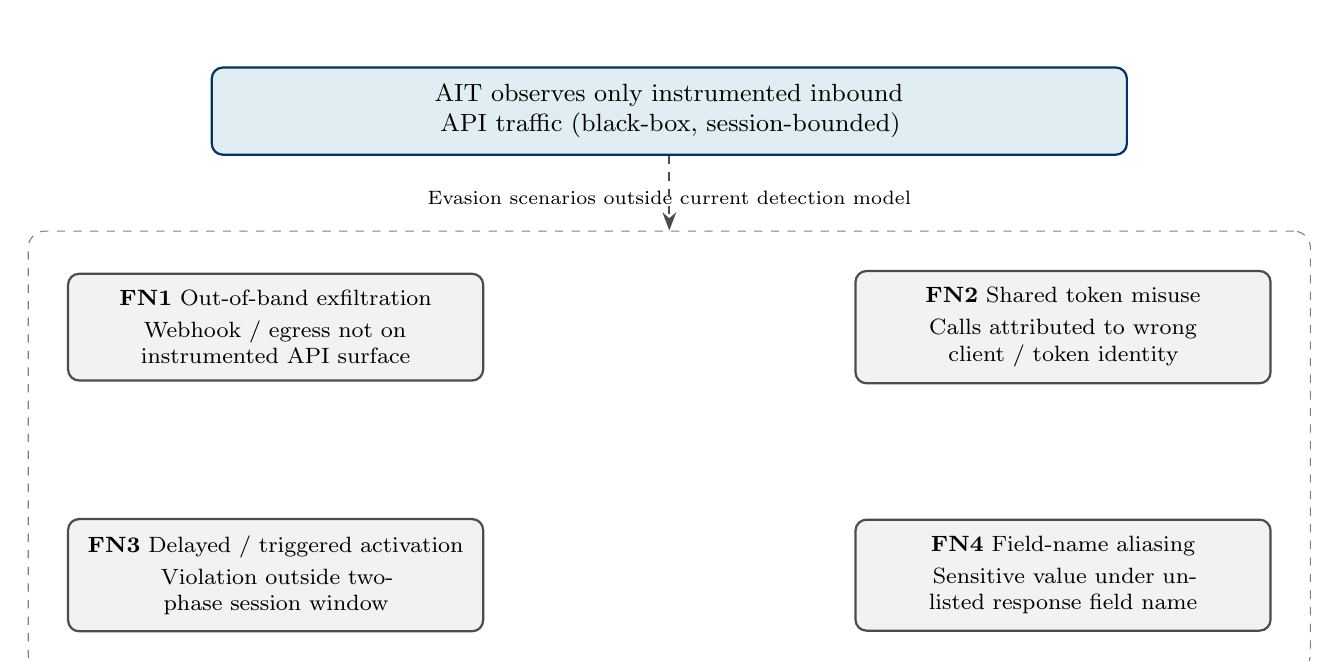
\begin{tikzpicture}[font=\footnotesize]
        \node[fnbox, text width=4.85cm] (fn1) at (-5.0, 0) {%
            \textbf{FN1} Out-of-band exfiltration\\[2pt]
            Webhook / egress not on instrumented API surface};
        \node[fnbox, text width=4.85cm] (fn2) at (5.0, 0) {%
            \textbf{FN2} Shared token misuse\\[2pt]
            Calls attributed to wrong client / token identity};
        \node[fnbox, text width=4.85cm] (fn3) at (-5.0, -3.15) {%
            \textbf{FN3} Delayed / triggered activation\\[2pt]
            Violation outside two-phase session window};
        \node[fnbox, text width=4.85cm] (fn4) at (5.0, -3.15) {%
            \textbf{FN4} Field-name aliasing\\[2pt]
            Sensitive value under unlisted response field name};
        \node[draw=black!50, dashed, rounded corners=6pt, inner sep=14pt,
              fit=(fn1)(fn2)(fn3)(fn4), label={[font=\scriptsize, yshift=6pt]above:%
              Evasion scenarios outside current detection model}] (boundary) {};
        \node[aitobs, text width=11.2cm, above=0.95cm of boundary.north] (scope) {%
            AIT observes only instrumented inbound API traffic (black-box, session-bounded)%
        };
        \draw[arrow, dashed] (scope.south) -- (boundary.north);
    \end{tikzpicture}
    \caption{False-negative evasion scenarios beyond the current black-box, session-bounded model.
             These are design boundaries, not implementation defects.}
    \label{fig:fn-overview}
\end{figure}

\section{FN1 --- Out-of-Band Exfiltration}

An integration that accesses authorised endpoints but exfiltrates data via a separate webhook,
outbound HTTP request, or side channel will not be detected, as AIT observes only inbound API
calls to the instrumented SaaS surface. \textbf{Mitigation direction:} network egress monitoring
or outbound traffic analysis.

\section{FN2 --- Shared Token Misuse}

If two integrations share an OAuth token issued to a different client ID, AIT --- which attributes
calls by run ID, not token identity --- will not associate the unauthorised calls with the IUT.
\textbf{Mitigation direction:} per-integration token isolation at the platform level.

\section{FN3 --- Time-Delayed or Trigger-Based Activation}

An integration that activates unauthorised access after a fixed delay (e.g., 30 days
post-installation) or via an external command-and-control signal will evade the two-phase model,
which is bounded by the test session duration. \textbf{Mitigation direction:} continuous runtime
monitoring beyond point-in-time assessment.

\section{FN4 --- Response-Field Aliasing}

If an integration reads sensitive data from a field whose name does not match any token in
\texttt{sensitive\_markers} (e.g., a renamed or obfuscated field in a non-standard API response
schema), taint detection will fail. \textbf{Mitigation direction:} value-pattern matching in
addition to field-name matching; semantic field classification using NLP. The mock harness
reproduces this miss explicitly (Section~5.6, FN4 negative row).

These false negative cases are not implementation bugs but fundamental constraints of the
black-box, session-bounded, field-name-based detection model.

% ══════════════════════════════════════════════════════════════════════════════
\chapter{Limitations and Future Scope}

\section{Current Limitations}

\textbf{L1: External Validity.}
Primary evidence comprises mock scenarios, replayed public incidents, and a live probe design
for two sandbox accounts (GitHub and Notion) whose Task~6 empirical rows are
\texttt{NOT RUN}/\textbf{BLOCKED} without credentials. The framework has not been
evaluated tenant-wide on live production SaaS platforms; this remains the primary limitation.

\textbf{L2: Evaluation Scale.}
The offline mock corpus comprises 16~YAML scenarios: 6~CRM (3~isolation + 3~controls) and
10~platform-inspired (7~violation-oriented + 3~compliant controls); live sandbox plans exist but empirical runs are
blocked. A larger, more adversarial test suite is
needed.

\textbf{L3: Scoring Model.}
The heuristic design-constant weights are justified and sensitivity-analysed, but not empirically validated
against a ground-truth dataset of real integration violations. Allow/deny live policy checks remain
future work / not yet implemented.

\textbf{L4: Two-Phase Model Coverage.}
Real integrations may exhibit variation across more state dimensions than two phases can capture
(FN3).

\textbf{L5: In-Memory State.}
Non-persistent and not multi-process safe; a production deployment requires a persistent backend
(PostgreSQL or Redis).

\textbf{L6: Live Runner Authentication.}
The current bearer-token auth shape covers GitHub, Notion, Slack, and Google; platforms with
non-standard auth conventions require per-platform adapters.

\section{Future Scope}

\textbf{F1: Live Platform Evaluation at Scale.}
Expand live sandbox evaluation to Slack, GitHub, and Google Workspace at broader scale --- the
single highest-impact next step.

\textbf{F2: Automatic Policy Inference.}
Develop automatic policy inference from OpenAPI specifications and historical access logs,
reducing the burden of manually authoring \texttt{TargetConfig} YAML files.

\textbf{F3: ML-Based Anomaly Detection.}
Implement ML-based anomaly detection for access patterns not requiring pre-specified allowlists,
enabling detection of novel over-scope behaviour without explicit policy definition.

\textbf{F4: Multi-Phase State-Machine-Guided Execution.}
Replace the two-phase model with a state-machine-guided execution engine covering richer
behavioural spaces, addressing FN3.

\textbf{F5: Outbound Traffic Monitoring.}
Add network egress monitoring to address FN1 (out-of-band exfiltration).

\textbf{F6: Value-Pattern Taint Matching.}
Implement value-pattern taint matching (regular expressions, semantic field classification via
NLP) in addition to field-name matching, addressing FN4.

\textbf{F7: CI/CD Pipeline Integration.}
Formalise CI/CD pipeline integration enabling automated regression testing on each integration
deployment, gating merges when policy drift is detected.

\textbf{F8: Empirical Risk-Weight Calibration.}
Validate heuristic design-constant weights against a labelled dataset of real integration violations.

% ══════════════════════════════════════════════════════════════════════════════
\chapter{Conclusion}

The Adversarial Integration Tester (AIT) closes a gap left by server-focused fuzzers and static
scope tools: black-box reconciliation of observed integration traffic against an explicit policy
artifact. The design combines an integration-centric test subject, dual-phase stimulation for C3,
and instrumentation-free taint markers for C2.

A live SaaS evaluation pipeline (\texttt{ait/live\_runner.py}) is implemented for
instrumented sandbox probes, but GitHub and Notion Task~6 results remain
\texttt{NOT RUN}/\textbf{BLOCKED} without credentials---no live risk scores are claimed.

The Hardware and Software Requirements chapter (Chapter~\ref{ch:hwsw}) establishes that AIT
can be deployed on commodity hardware using an entirely open-source Python stack, with clear
upgrade paths to production-grade persistent backends and CI/CD integration.

Claims are scoped to controlled mocks, live sandbox evaluations, optional smoke probes, and
replayed public incidents; false-negative analysis bounds guarantees. Broader tenant-scale
validation remains future work. This work establishes integration-policy conformance as a
first-class security property in SaaS ecosystems, tightening least-privilege practice under
zero-trust assumptions and complementing --- not replacing --- existing server-side fuzzing and
static OAuth auditing tools.

% ══════════════════════════════════════════════════════════════════════════════
\begin{thebibliography}{35}

\bibitem{csa2023}
Cloud Security Alliance, ``SaaS Security Survey Report,'' 2023.

\bibitem{cisa2020}
CISA, ``Alert (AA20-352A): Advanced Persistent Threat Compromise of Government Agencies,
Critical Infrastructure, and Private Sector Organizations,'' Dec.\ 2020.

\bibitem{okta2022}
Okta, ``Okta Security Incident: January 2022,'' Security Advisory, Mar.\ 2022.

\bibitem{circleci2023}
CircleCI, ``CircleCI Security Incident Disclosure and Recommended Customer Actions,'' Jan.\ 2023.
\url{https://circleci.com/blog/jan-4-2023-security-alert/}

\bibitem{github2022}
GitHub, ``Security Alert: Attack Campaign Involving Stolen OAuth User Tokens Issued to Two
Third-Party Integrators,'' Apr.\ 2022.
\url{https://github.blog/2022-04-15-security-alert-stolen-oauth-user-tokens/}

\bibitem{aliyu2023}
F.\ Aliyu, C.\ Benson, and M.\ Ismail, ``Over-Privileged OAuth Grants in Enterprise SaaS:
Measurement and Risk Characterization,'' \textit{IEEE Trans.\ Dependable Secure Comput.},
vol.\ 20, no.\ 4, pp.\ 3211--3225, Jul./Aug.\ 2023.

\bibitem{rfc6749}
D.\ Hardt, Ed., ``The OAuth 2.0 Authorization Framework,'' RFC 6749, IETF, Oct.\ 2012.

\bibitem{rfc7636}
N.\ Sakimura, J.\ Bradley, and N.\ Agarwal, ``Proof Key for Code Exchange by OAuth Public
Clients,'' RFC 7636, IETF, Sep.\ 2015.

\bibitem{oidc2014}
N.\ Sakimura et al., ``OpenID Connect Core 1.0,'' OpenID Foundation, Nov.\ 2014.

\bibitem{fett2017}
D.\ Fett, R.\ K\"{u}sters, and G.\ Schmitz, ``The Web SSO Standard OpenID Connect:
In-Depth Formal Security Analysis and Security Guidelines,'' \textit{Proc.\ IEEE CSF}, 2017.

\bibitem{felt2012}
A.\ P.\ Felt, E.\ Ha, S.\ Egelman, A.\ Haney, E.\ Chin, and D.\ Wagner, ``Android
Permissions: User Attention, Comprehension, and Behavior,'' \textit{Proc.\ SOUPS}, 2012.

\bibitem{owaspapi2023}
OWASP, ``OWASP API Security Top 10 -- 2023 Edition.''
\url{https://owasp.org/www-project-api-security/}

\bibitem{mainka2022}
C.\ Mainka, V.\ Mladenov, J.\ Schwenk, and T.\ Wich, ``SoK: Benchmarking the Effectiveness
of OAuth Grant Type Enforcement Across Major SaaS Providers,'' \textit{Proc.\ ACM CCS}, 2022.

\bibitem{decarne2023}
X.\ De Carne de Carnavalet and P.\ C.\ van Oorschot, ``Third-Party Application Permission
Practices: A Large-Scale Analysis of OAuth over Major Identity Providers,''
\textit{Proc.\ USENIX Security}, 2023.

\bibitem{boucher2024}
T.\ Boucher, A.\ Kharraz, and E.\ Kirda, ``Scope Guard: Static Policy Enforcement for SaaS
Integration Permission Graphs,'' \textit{Proc.\ NDSS}, 2024.

\bibitem{lundberg2024}
E.\ Lundberg, M.\ Ekstedt, and R.\ Lagerstr\"{o}m, ``Runtime OAuth Scope Enforcement via
Transparent API Proxy Middleware,'' \textit{Proc.\ IEEE EuroS\&P}, 2024.

\bibitem{afl}
M.\ Zalewski, ``American Fuzzy Lop (AFL),'' 2014.
\url{https://lcamtuf.coredump.cx/afl/}

\bibitem{boofuzz}
J.\ Pereyda, ``Boofuzz: A Fork and Fix of Sulley.''
\url{https://github.com/jtpereyda/boofuzz}

\bibitem{restler2019}
V.\ Atlidakis, P.\ Godefroid, and M.\ Polishchuk, ``RESTler: Stateful REST API Fuzzing,''
\textit{Proc.\ ICSE}, 2019.

\bibitem{evomaster2019}
A.\ Arcuri, ``RESTful API Automated Test Case Generation with EvoMaster,''
\textit{ACM Trans.\ Softw.\ Eng.\ Methodol.}, vol.\ 28, no.\ 1, 2019.

\bibitem{atlidakis2020}
V.\ Atlidakis, P.\ Godefroid, and M.\ Polishchuk, ``Checking Security Properties of Cloud
Service REST APIs,'' \textit{Proc.\ IEEE S\&P}, 2020.

\bibitem{yang2011}
X.\ Yang, Y.\ Chen, E.\ Eide, and J.\ Regehr, ``Finding and Understanding Bugs in C
Compilers,'' \textit{Proc.\ PLDI}, 2011.

\bibitem{petsios2017}
T.\ Petsios, J.\ Zhao, A.\ D.\ Keromytis, and S.\ Jana, ``SlowFuzz: Automated
Domain-Independent Detection of Algorithmic Complexity Vulnerabilities,''
\textit{Proc.\ CCS}, 2017.

\bibitem{kim2022}
S.\ Kim, Y.\ Lee, and J.\ Choi, ``DiffMicro: Differential Testing for Semantic Consistency
in Microservice API Evolution,'' \textit{Proc.\ IEEE ICWS}, 2022.

\bibitem{benamara2020}
F.\ Benamara, N.\ Mager, and M.\ Dacier, ``DPIFuzz: A Differential Fuzzing Framework to
Detect DPI Elusion Strategies for QUIC,'' \textit{Proc.\ ACSAC}, 2020.

\bibitem{bulekov2023}
A.\ Bulekov, B.\ Das, S.\ Hajnoczi, and M.\ Egele, ``Fuzztruction: Using Fault Injection to
Hack Fuzzing Mutators,'' \textit{Proc.\ USENIX Security}, 2023.

\bibitem{livshits2005}
V.\ B.\ Livshits and M.\ S.\ Lam, ``Finding Security Vulnerabilities in Java Applications
with Static Analysis,'' \textit{Proc.\ USENIX Security}, 2005.

\bibitem{clause2007}
J.\ Clause, W.\ Li, and A.\ Orso, ``Dytan: A Generic Dynamic Taint Analysis Framework,''
\textit{Proc.\ ISSTA}, 2007.

\bibitem{taintdroid2014}
W.\ Enck et al., ``TaintDroid: An Information-Flow Tracking System for Realtime Privacy
Monitoring on Smartphones,'' \textit{ACM Trans.\ Comput.\ Syst.}, vol.\ 32, no.\ 2, 2014.

\bibitem{pan2022}
X.\ Pan, Y.\ Zhang, and M.\ Grace, ``SynthAPI: Privacy-Preserving Synthetic Data Generation
for API Security Testing,'' \textit{Proc.\ ACM CODASPY}, 2022.

\bibitem{nist800207}
S.\ Rose, O.\ Borchert, S.\ Mitchell, and S.\ Connelly, ``Zero Trust Architecture,''
NIST Special Publication 800-207, Aug.\ 2020.

\bibitem{ding2023}
Y.\ Ding, R.\ Phan, and T.\ P\"{o}ppelmann, ``Continuous Authorization for Third-Party SaaS
Integrations under Zero Trust,'' \textit{Proc.\ IEEE CloudCom}, 2023.

\bibitem{wermke2022}
D.\ Wermke et al., ``A Large Scale Investigation of Obfuscation Use in Google Play,''
\textit{Proc.\ USENIX Security}, 2022.

\bibitem{chandramouli2023}
R.\ Chandramouli, ``SaaS Security Posture Management: Taxonomy, Challenges, and Research
Directions,'' NIST Internal Report 8467, 2023.

\bibitem{cvss31}
FIRST.Org, ``Common Vulnerability Scoring System v3.1: Specification Document,'' 2019.
\url{https://www.first.org/cvss/specification-document}

\end{thebibliography}

\end{document}
